\documentclass[class=report,crop=false]{standalone}
\usepackage[screen]{../exo7book}

% Commande ponctuelle
\newcommand{\alenvers}[1]{\rotatebox[origin=c]{180}{#1}}
\newcommand{\vect}{\overrightarrow}

\begin{document}

%====================================================================
\chapitre{Calcul formel}
%====================================================================

%\insertvideo{kvviYsb9Ltk}{partie 6a. Courbes et surfaces}

%\insertvideo{ttiZ7bDXeEA}{partie 6b. Courbes et surfaces}


%%%%%%%%%%%%%%%%%%%%%%%%%%%%%%%%%%%%%%%%%%%%%%%%%%%%%%%%%%%%%%%%
\setcounter{section}{5}
\section{Courbes et surfaces}

La visualisation est une étape importante dans l'élaboration 
des preuves en mathématiques. L'avènement des logiciels de calcul 
formel possédant une interface graphique évoluée a 
rendu cette phase attrayante. Nous allons explorer 
les possibilités graphiques offertes par \Sage.
Nous avons déjà vu comment tracer les graphes de fonctions avec la commande \codeinline{plot}
(voir \og Premiers pas avec \Sage\ \fg{}), par exemple \codeinline{plot(sin(x)*exp(x),(x,-3,3))}
trace le graphe de la fonction $f(x)=\sin(x)\exp(x)$ sur l'intervalle $[-3,3]$.
\begin{center}
 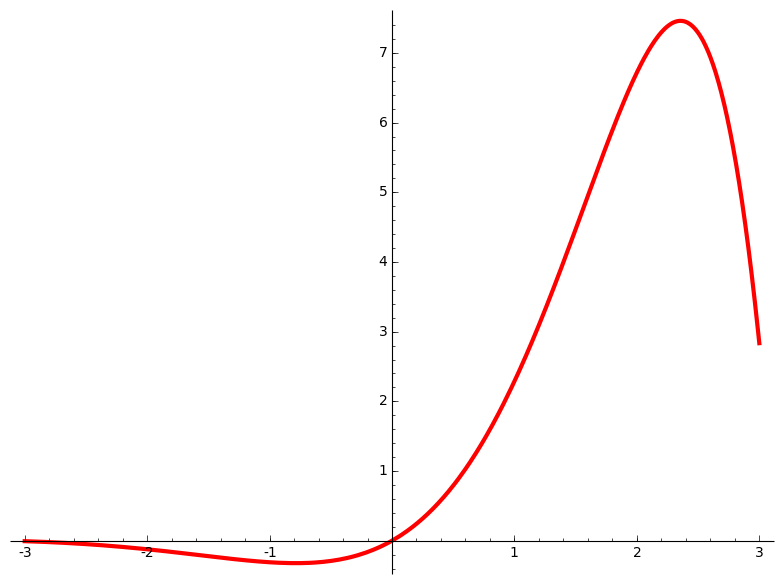
\includegraphics[scale=0.3]{figures/intro_courbes} 
\end{center}

En plus des graphes de fonctions, \Sage\ sait tracer des courbes et des surfaces par d'autres méthodes.

%--------------------------------------------------------
\subsection{Courbes paramétrées}

La commande \codeinline{parametric_plot((f(t), g(t)), (t, a, b))} 
permet de tracer la courbe paramétrée plane donnée par les points 
de coordonnées $(f(t), g(t))$ lorsque le paramètre $t$ varie 
dans l'intervalle $[a,b]$. 
Commençons par la lemniscate de Bernoulli :


\begin{center}
 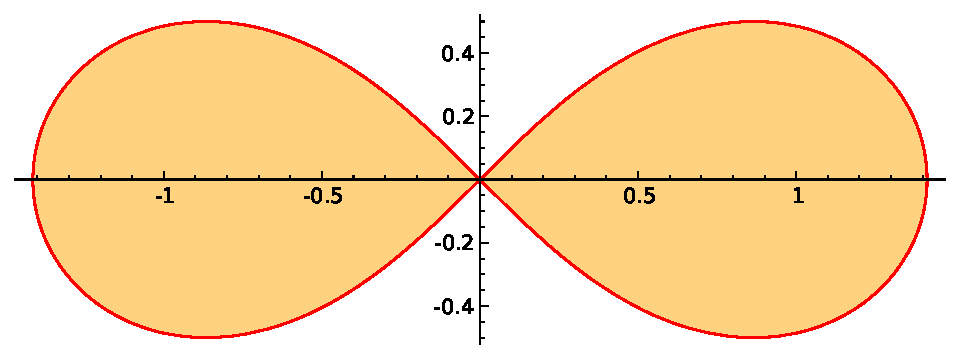
\includegraphics[scale=0.7]{figures/lemniscate_bernoulli} 
\end{center}




\insertcode{algos/lemniscate_bernoulli-tex.sage}{lemniscate-bernoulli.sage}


\begin{tp}
\sauteligne
\begin{enumerate}
  \item Tracer la spirale de Fermat d'équation
  $$\left\{
\begin{array}{l}
x(t)=\sqrt t \cos t\\[1mm]
y(t)=\sqrt t \sin t
\end{array}
\right. \qquad t \in \Rr_+.$$
  \item Tracer la courbe du papillon
  $$\left\{
\begin{array}{l}
x(t) = \sin(t)\left(\exp(\cos(t))-2\cos(4t)-\sin^5\left(\frac{t}{12}\right)\right)\\[3mm]
y(t) = \cos(t)\left(\exp(\cos(t))-2\cos(4t)-\sin^5\left(\frac{t}{12}\right)\right)
\end{array}
\right. \qquad t \in \Rr.$$
\end{enumerate} 
\end{tp}


\begin{center}
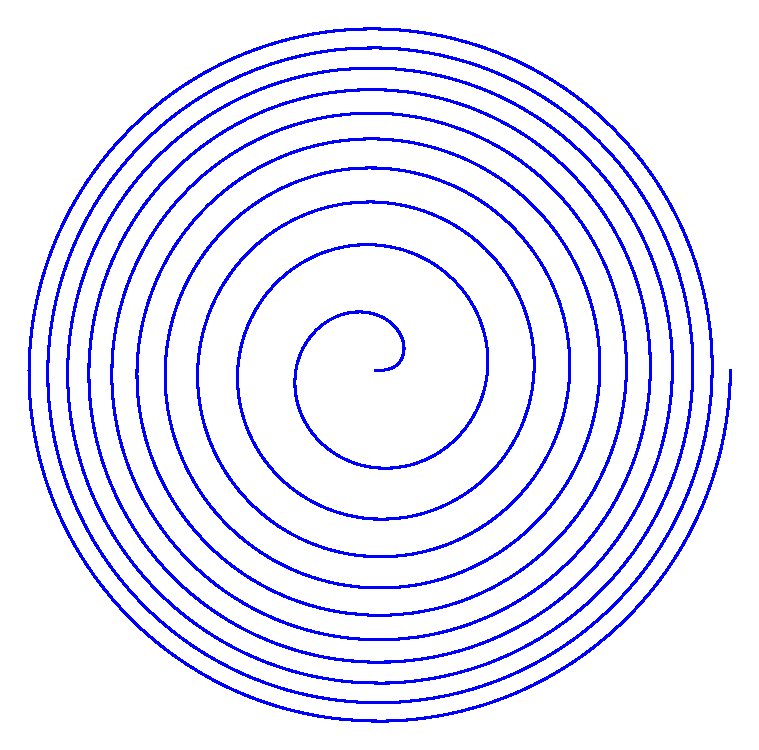
\includegraphics[scale=0.5]{figures/fermat_spiral}\quad
\includegraphics[scale=0.4]{figures/butterfly_curve}  
\end{center}


Les commandes de tracé possèdent de nombreuses options, 
qu'on pourra découvrir grâce 
à la commande \codeinline{help(parametric_plot)}. 
Par exemple :
\begin{itemize}
  \item Imposer un repère orthonormé : \codeinline{aspect_ratio = 1}

  \item Nombre de points pour le tracé : \codeinline{plot_points = 500}
    
  \item Ne pas afficher les axes : \codeinline{axes = False}
  
  \item Afficher une grille : \codeinline{gridlines = True}
    
  \item Couleur du trait : \codeinline{color = 'red'},

  \item Remplir l'intérieur : \codeinline{fill = True},

  \item Couleur du remplissage : \codeinline{fillcolor = 'orange'}.
\end{itemize}

% \insertcode{algos/fermat_spiral.sage}{fermat-spiral.sage}
% \insertcode{algos/butterfly_curve.sage}{butterfly-curve.sage}

%--------------------------------------------------------
\subsection{Courbes en coordonnées polaires}

Les courbes en coordonnées polaires sont tracées grâce à la 
commande \codeinline{polar_plot(r(t),(t,a,b))}, qui produira 
l'ensemble des points de coordonnées polaires $[r(t):t]$ pour 
$t$ variant dans l'intervalle $[a,b]$.
Voici le folium de Dürer d'équation 
$r(t) = \sin \frac t 2$, $t \in \Rr$.


\begin{center}
 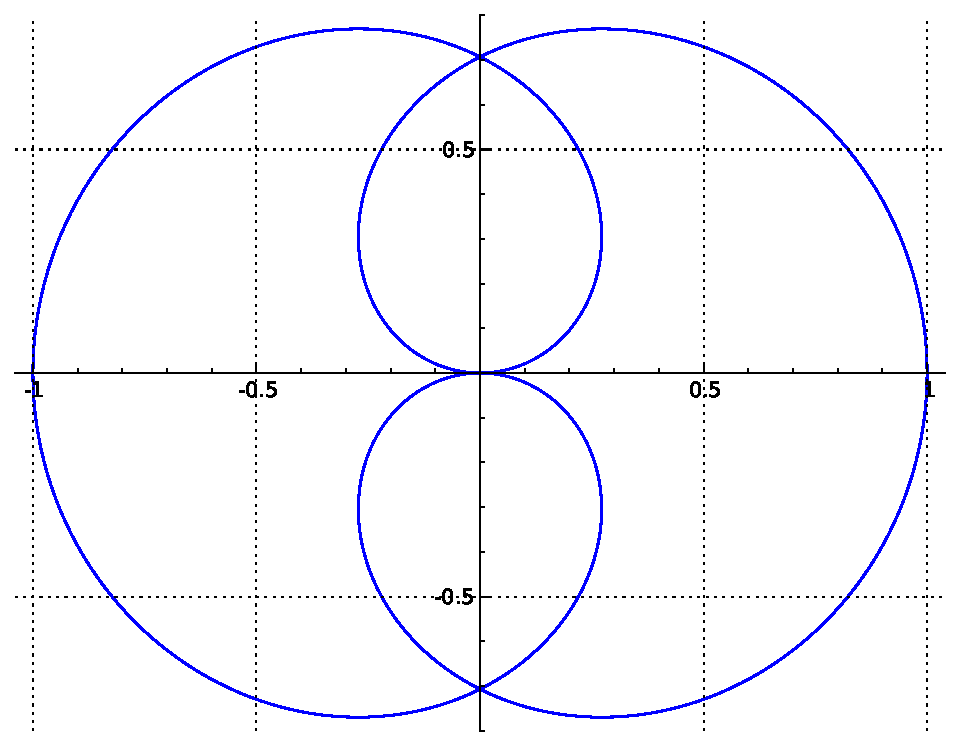
\includegraphics[scale=0.5]{figures/durer_folium} 
\end{center}


\insertcode{algos/durer_folium-tex.sage}{durer-folium.sage}

%Les options sont sensiblement les mêmes que celles 
% de la commande \codeinline{parametric_plot}, 
% on pourra y accéder grâce à la commande 
% \codeinline{help(polar_plot)}. 
% Voici quelques exemples.




\begin{tp}
\sauteligne
\begin{enumerate}
  \item Tracer la courbe du Lituus d'équation polaire 
  $$r(t)^2 = \frac{1}{t} \qquad t \in \Rr^*.$$
  \item Tracer la cochléoïde d'équation polaire 
  $$r(t) = \frac{\sin t}{t} \qquad t \in \Rr^*.$$
\end{enumerate} 
\end{tp}

Indications : on peut définir deux graphes \codeinline{G1} et 
\codeinline{G2} pour chacun des intervalles de définition. On superpose
les graphes avec \codeinline{G = G1 + G2}, puis on les affiche avec 
\codeinline{G.show()}.


\begin{center}
  \begin{minipage}{0.49\textwidth}
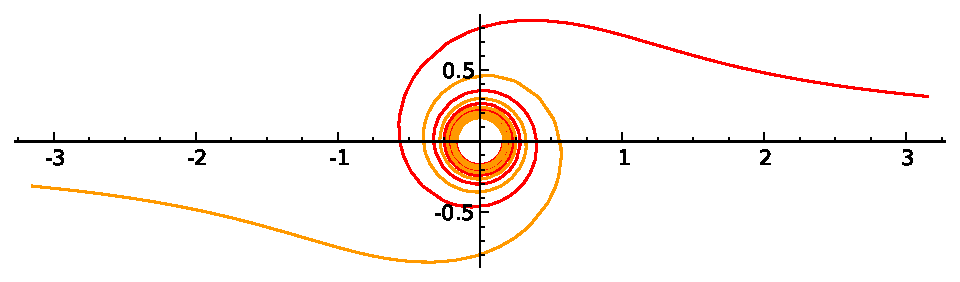
\includegraphics[scale=0.5]{figures/lituus}  
\end{minipage}
\begin{minipage}{0.49\textwidth}
\qquad\qquad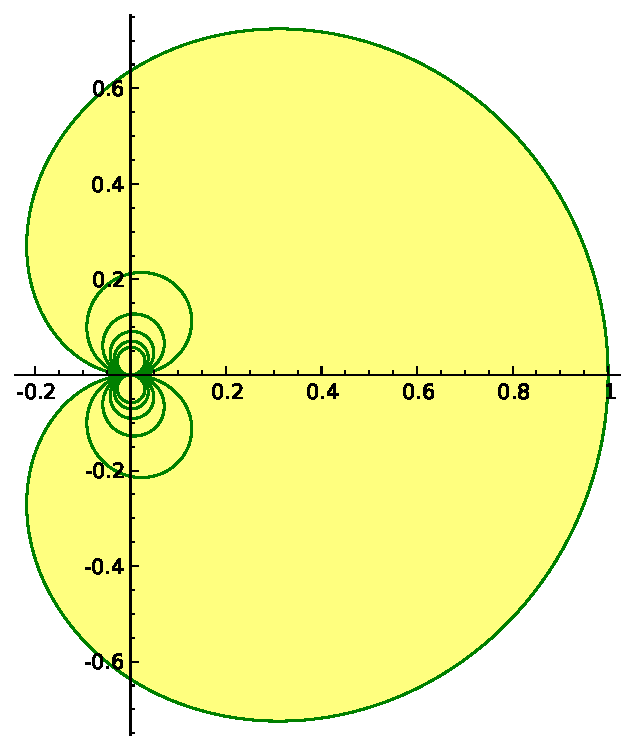
\includegraphics[scale=0.5]{figures/cochleoid}  
\end{minipage}
\end{center}



% \insertcode{algos/lituus.sage}{lituus.sage}
% \insertcode{algos/cochleoid.sage}{cochleoid.sage}



%--------------------------------------------------------
\subsection{Courbes définies par une équation}

Une courbe peut avoir plusieurs types de représentations, comme par exemple
un cercle d'équation paramétrique $(\cos t,\sin t)$ ou d'équation implicite
$x^2+y^2 = 1$.
La commande \\
\centerline{\codeinline{implicit_plot(f(x, y), (x, a, b), (y, c, d))} }
permet de tracer l'ensemble des couples $(x,y)$ 
dans $[a,b]\times[c,d]$ qui sont solutions de l'équation 
$f(x,y)=0$. Voici une autre courbe de papillon, cette fois algébrique. 

\insertcode{algos/butterfly_curve_algebraic-tex.sage}{butterfly-curve-algebraic.sage}


Noter comment il est possible de sauvegarder une image du tracé dans un fichier externe.


\begin{center}
  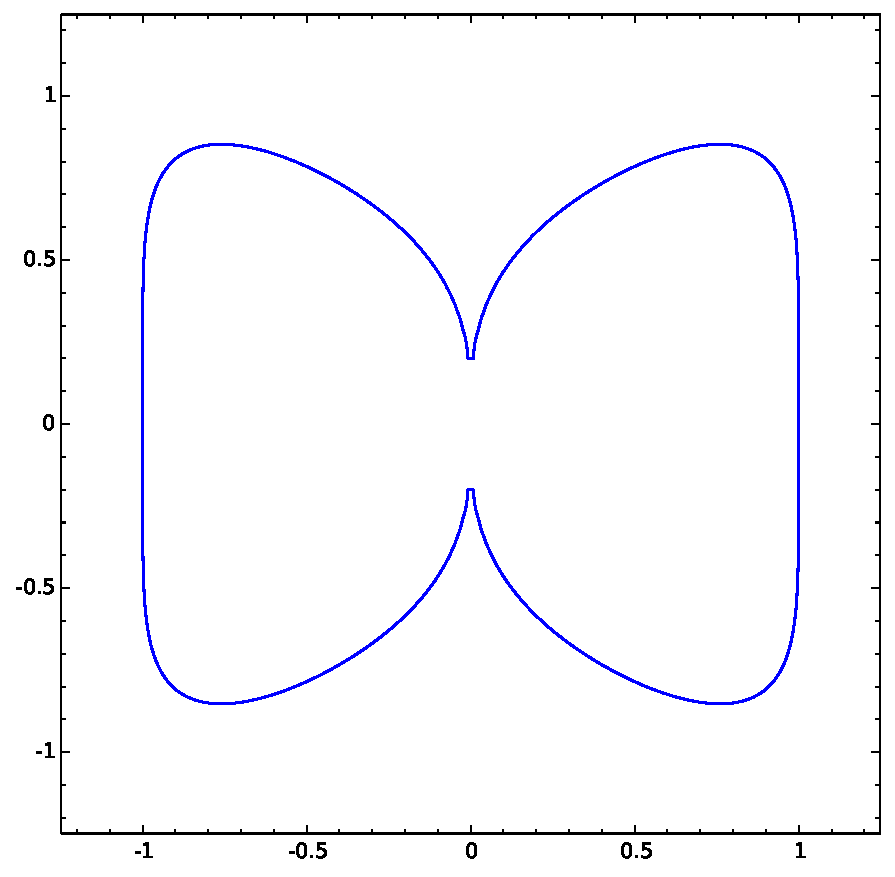
\includegraphics[scale=0.4]{figures/butterfly_curve_algebraic}
\end{center}

\begin{tp}
\sauteligne
\begin{enumerate}
  \item Construire une liste contenant les représentations graphiques de la courbe définie par
  $$y^2-x^3+x+c = 0$$
  lorsque le paramètre $c$ parcoure l'intervalle $[-1, 1]$ par pas de $0.1$.
  \item \`A l'aide de la commande \codeinline{animate}, 
  réaliser une animation qui affiche l'évolution de la courbe
  pour $c \in[-1,1]$.
\end{enumerate}
\end{tp}


\begin{center}
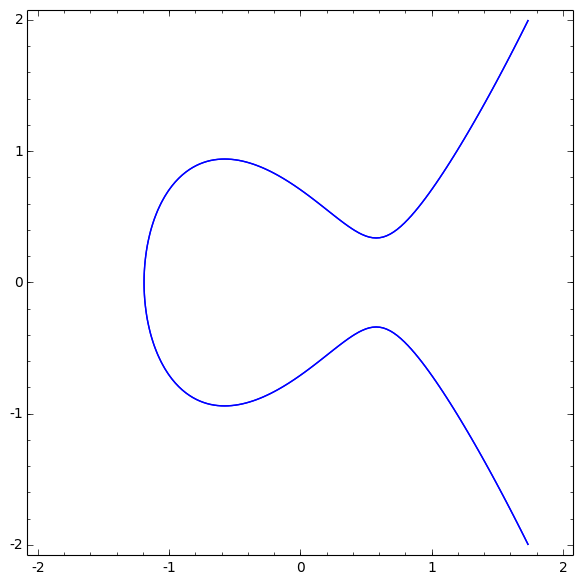
\includegraphics[scale=0.3]{figures/elliptic1}\quad
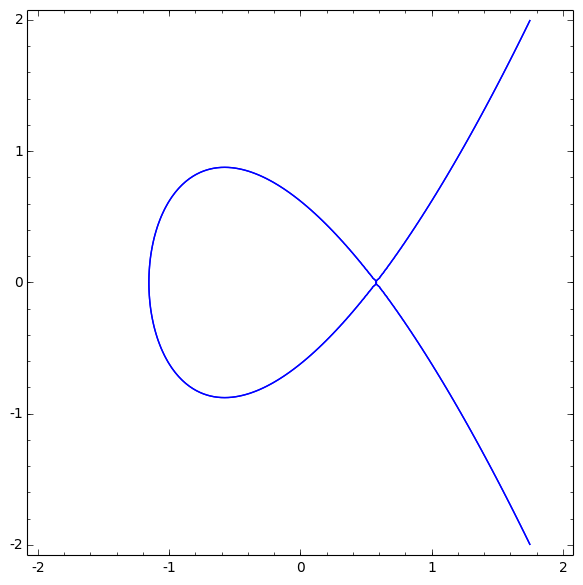
\includegraphics[scale=0.3]{figures/elliptic2}\quad
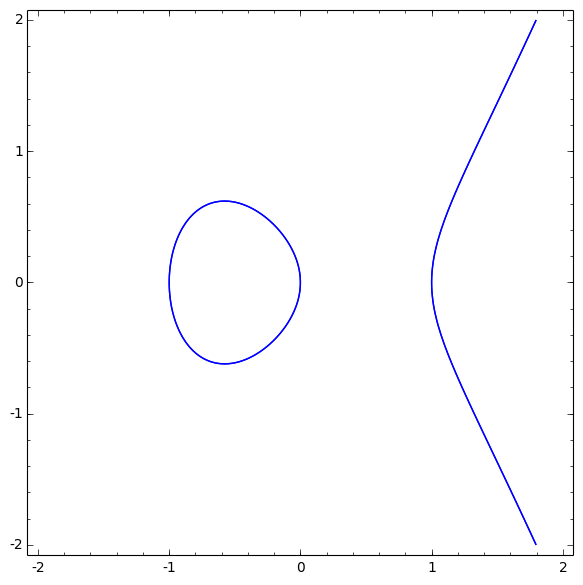
\includegraphics[scale=0.3]{figures/elliptic3}
\end{center}



%--------------------------------------------------------
\subsection{Courbes de l'espace}



La commande \codeinline{parametric_plot((x, y, z), (t, a, b))}, 
(ou bien \codeinline{parametric_plot3d()}) analogue à celle de la dimension $2$, 
trace la courbe paramétrée de 
l'espace donnée par les points de coordonnées $\big( x(t), y(t), z(t) \big)$ 
lorsque le paramètre $t$ varie dans l'intervalle $[a,b]$. 

\begin{tp}
Tracer la courbe d'Archytas d'équation paramétrique :
$$\left\{
\begin{array}{l}
x(t) = \cos^2 t \\[1mm]
y(t) = \cos t \sin t \\[1mm]
z(t) = \pm\sqrt{ \cos t(1-\cos t) }
\end{array}
\right.\qquad  t \in \big[-\tfrac\pi2,+\tfrac\pi2\big].$$
\end{tp}

%\insertcode{algos/archytas_curve.sage}{archytas-curve.sage}

Vous obtiendrez une figure qu'il est possible d'orienter dynamiquement 
avec la souris. Voici quelques-unes de ces vues.

\begin{center}
 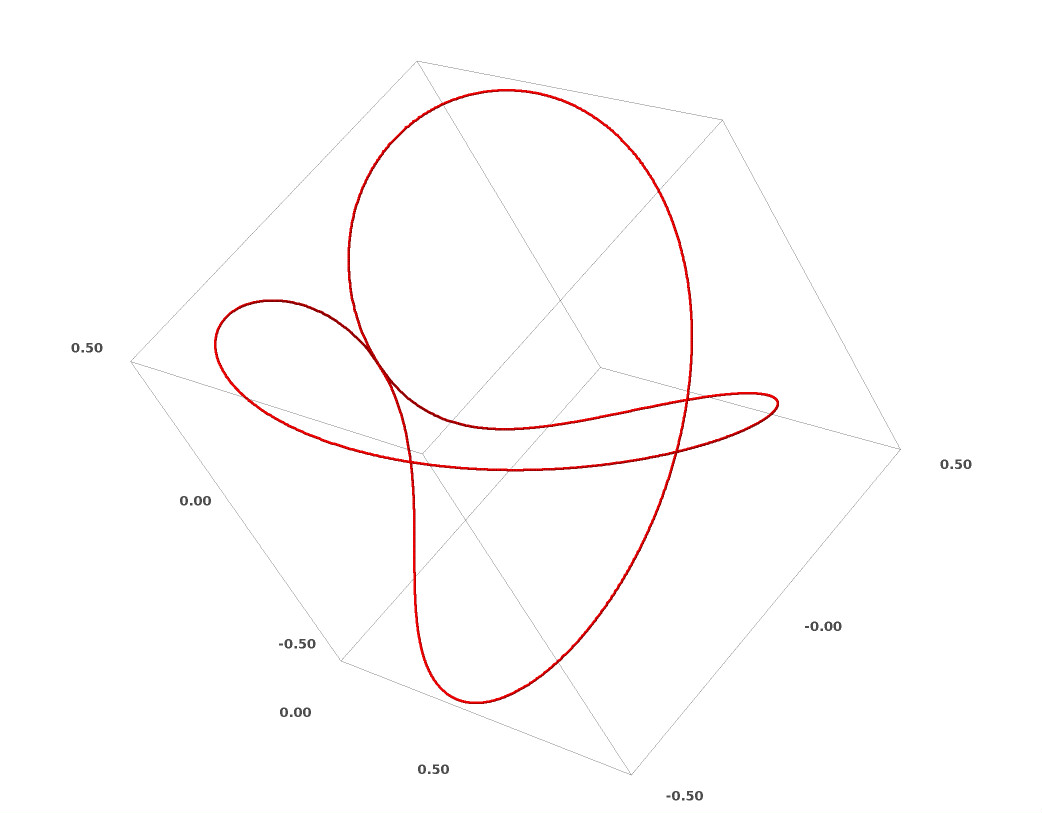
\includegraphics[scale=0.2]{figures/archytas_curve_new1.jpg} 
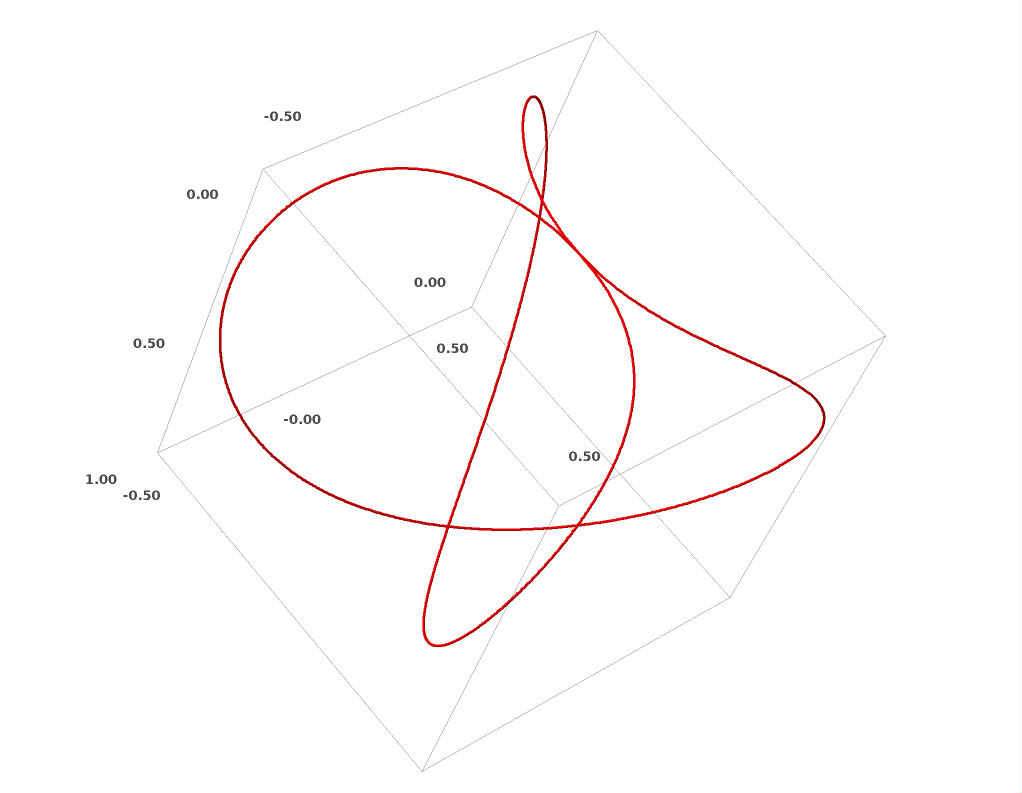
\includegraphics[scale=0.2]{figures/archytas_curve_new2.jpg}  
\end{center}




%--------------------------------------------------------
\subsection{Surfaces}


Découvrez, à l'aide de l'énoncé suivant, les différentes méthodes 
pour tracer des surfaces avec \Sage.

\begin{tp}
\sauteligne
\begin{enumerate}
  \item Tracer le graphe de la fonction $f(x,y)= x^2y^2-(x^2+y^2)^3$ définie
  sur $(x,y) \in [-1,1]\times[-1,1]$. Utiliser la fonction \codeinline{plot3d}.
  
  \item Tracer la surface d'Enneper
  définie par l'équation 
  $$\left( \frac{y^2-x^2}{2z}+\frac29z^2+\frac23\right)^3-
  6\left( \frac{y^2-x^2}{4z}-\frac14\big(x^2+y^2+\frac89z^2\big)+\frac29 \right)^2=0.$$
  Utiliser la fonction \codeinline{implicit_plot3d}.

  
  \item Tracer la nappe paramétrée définie par :
  $$\left\{
  \begin{array}{l}
  x(s,t) =  t^2 \cos s\\[1mm]
  y(s,t) =  s^2 \sin t\\[1mm]
  z(s,t) = \cos t+ \sin t
  \end{array}
  \right.\qquad  s \in \big[0,1\big], \quad t \in \big[-\pi,+\pi\big].$$
  Utiliser la fonction \codeinline{parametric_plot3d}.
  
  \item Tracer la surface paramétrée définie en coordonnées cylindriques par :
  $$r(\theta,z) = z^3 \cos \theta \qquad \theta \in [0,2\pi], \quad z \in [0,2].$$  
  Utiliser la fonction \codeinline{cylindrical_plot3d}.
  
  \item Tracer la surface paramétrée définie en coordonnées sphériques par 
  $$r(\theta,\phi)  = \theta \sin(2\phi) \qquad \theta \in [-1,2\pi], \quad  \phi \in [0,\pi].$$
  Utiliser la fonction \codeinline{spherical_plot3d}.  
\end{enumerate}
\end{tp}


%\insertcode{algos/surface.sage}{surface.sage}


\begin{center}
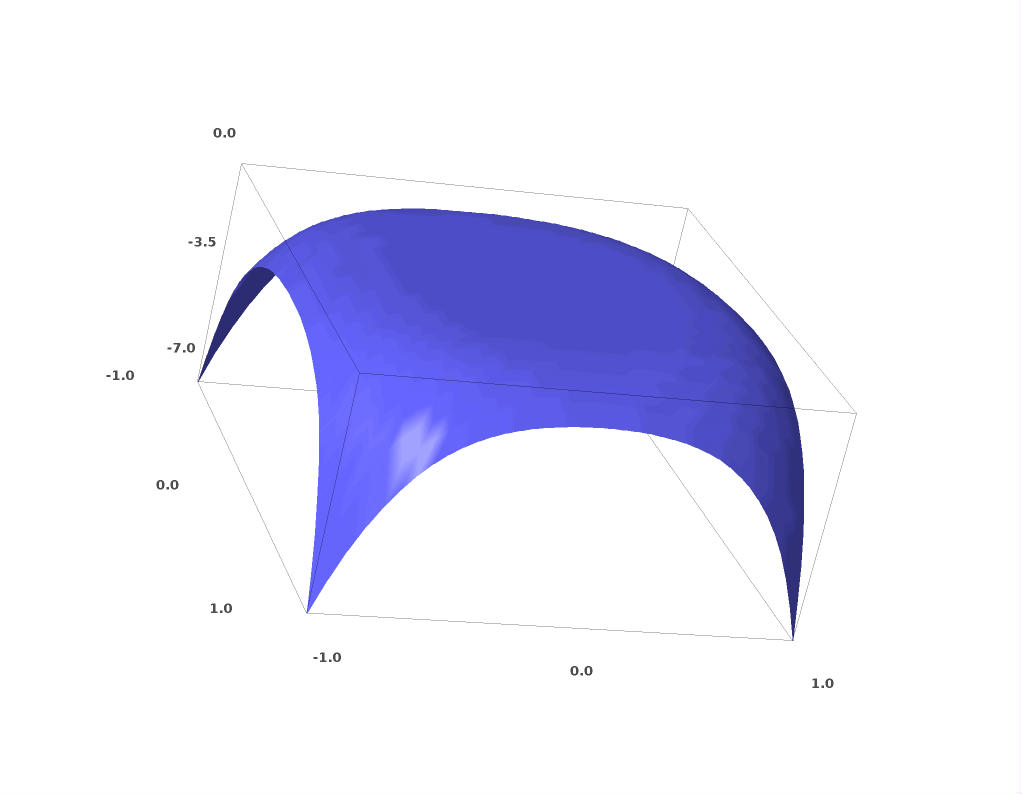
\includegraphics[scale=0.2]{figures/surface_1.jpg} 
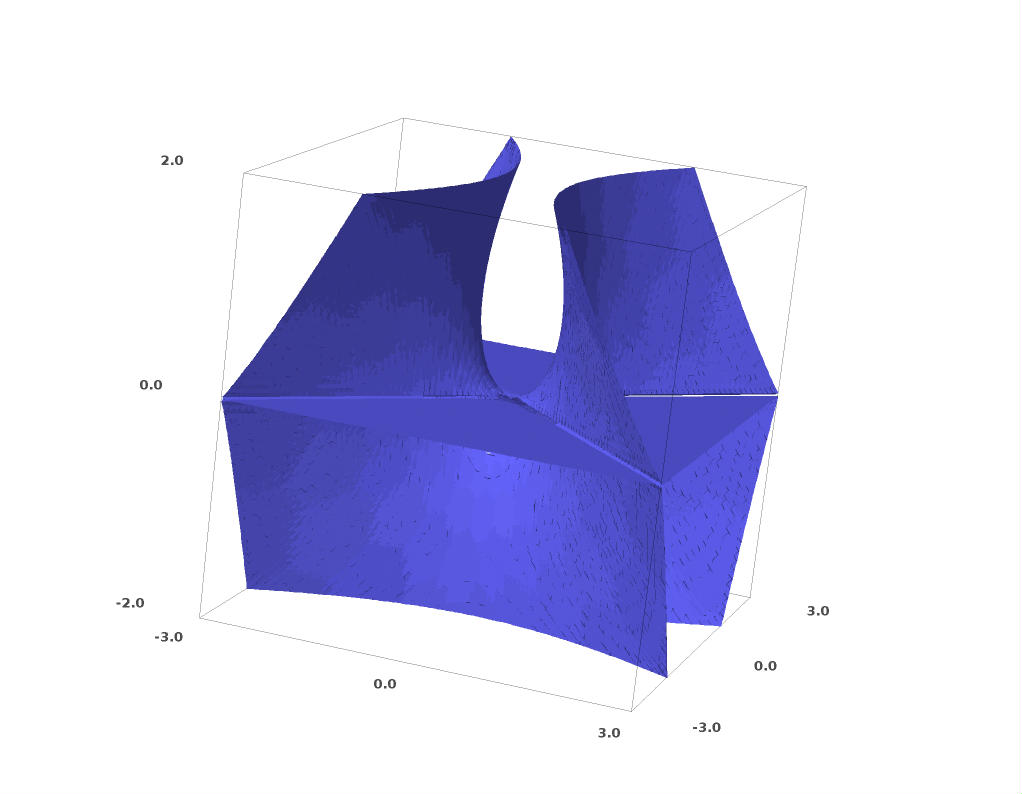
\includegraphics[scale=0.2]{figures/surface_2.jpg} \\ 
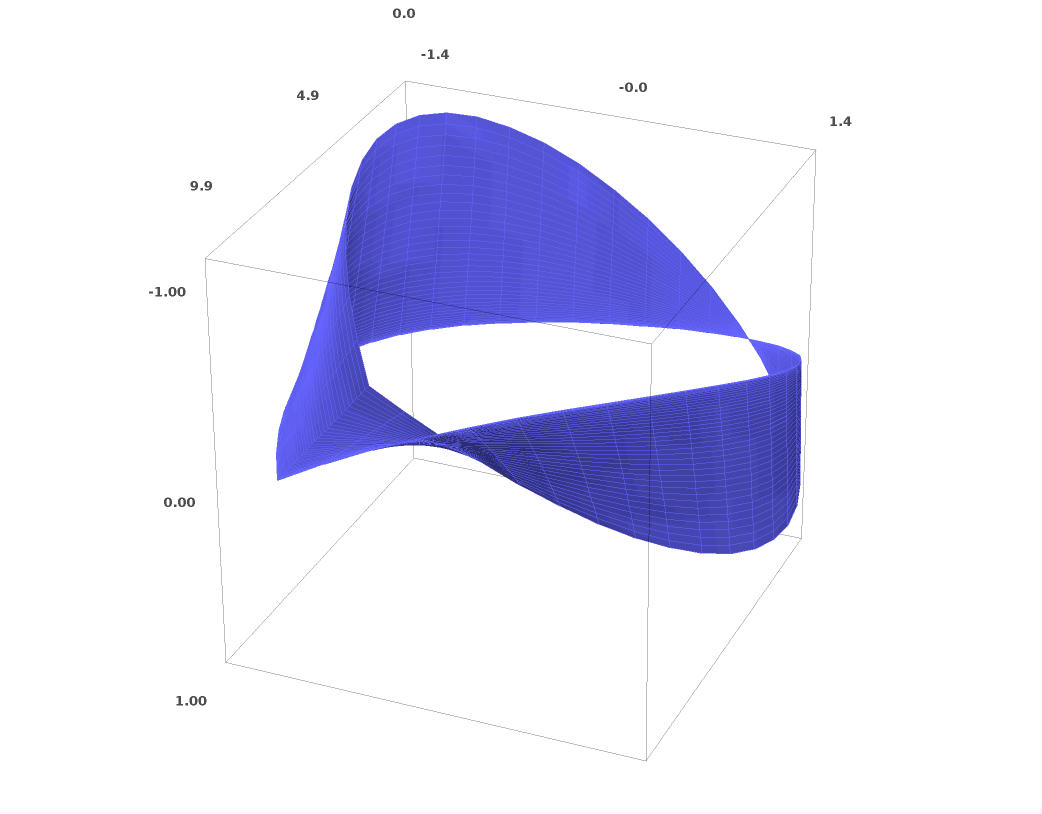
\includegraphics[scale=0.2]{figures/surface_3.jpg} \\
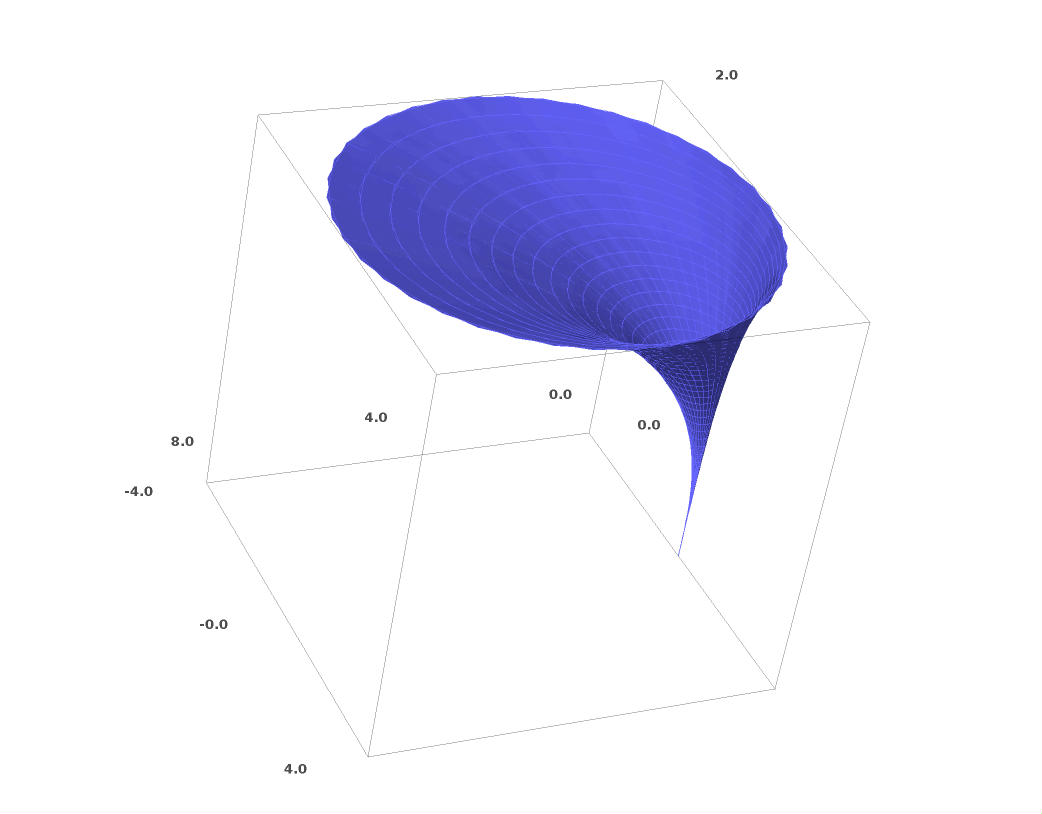
\includegraphics[scale=0.2]{figures/surface_4.jpg} 
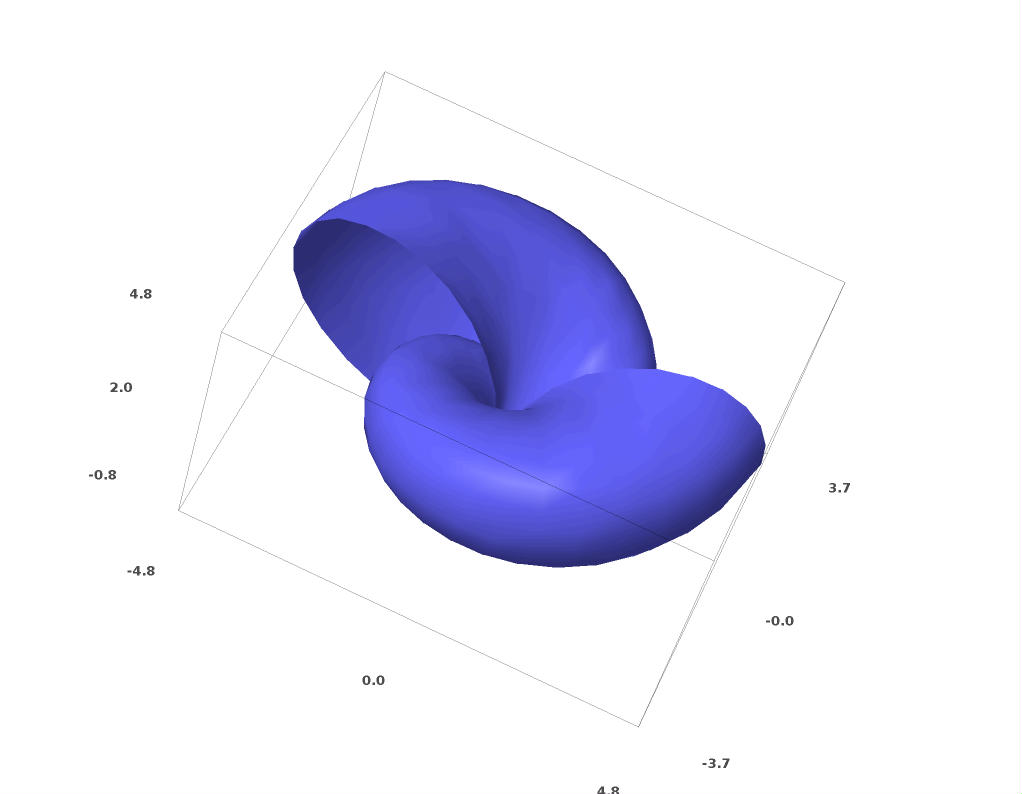
\includegraphics[scale=0.2]{figures/surface_5.jpg}  
\end{center}




%--------------------------------------------------------
\subsection{\'Etude d'une courbe paramétrée}

\begin{tp}
\'Etudier en détail la courbe paramétrée du plan définie par 
  $$\left\{
  \begin{array}{l}
  x(t) =  t^3-2t\\[1mm]
  y(t) =  t^2-t
  \end{array}
  \right.\qquad  t \in \Rr.$$
\begin{enumerate}
  \item Tracer la courbe.
  
  \item Trouver les points d'intersection de la courbe avec l'axe des ordonnées.
  
  \item Trouver les points en lesquels la tangente est verticale, puis horizontale.
  
  \item Trouver les coordonnées des points doubles.
\end{enumerate}
\end{tp}



\begin{center}
  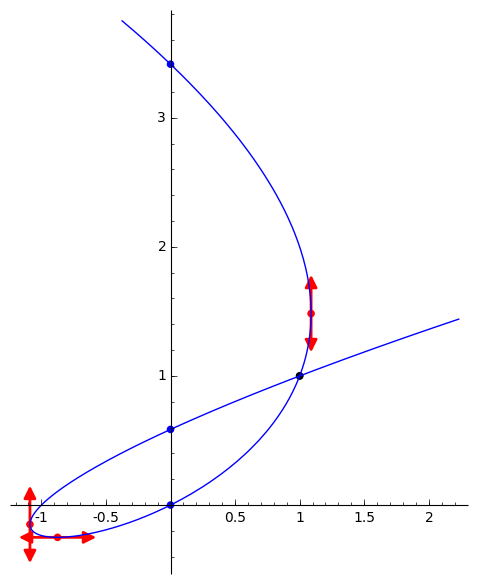
\includegraphics[scale=0.5]{figures/courbe.png} 
\end{center}



\begin{enumerate}
  \item La courbe a l'allure d'une boucle.
  \item On définit \codeinline{x = t^3-2*t} et \codeinline{y = t^2-t}.
On obtient les valeurs de $t$ correspondant aux points d'intersection de la courbe
avec l'axe $(x=0)$ en résolvant l'équation $x(t)=0$ : \codeinline{solve(x==0,t)}.
On obtient trois solutions $-\sqrt2$, $0$ et $+\sqrt2$ %$t \in \{-\sqrt2,0,+\sqrt2\}$ 
correspondant aux trois points
$\{(0,2+\sqrt2),(0,0),(0,2-\sqrt2)\}$
  
  \item On définit les fonctions dérivées $x'(t)$ et $y'(t)$
  par \codeinline{xx = diff(x,t)} et \codeinline{yy = diff(y,t)}. 
  Les valeurs de $t$ pour lesquelles la tangente à la courbe est verticale s'obtiennent en résolvant
  l'équation $x'(t)=0$, ce qui s'écrit \codeinline{solve(xx==0,t)}.
  
  \item Trouver les points doubles est souvent un calcul délicat (même pour un logiciel de calcul formel).
  Il s'agit ici de résoudre le système d'équations polynomiales :
   $$\left\{
  \begin{array}{l}
  x(s) =  x(t)\\[1mm]
  y(s) =  y(t)
  \end{array}
  \right.\qquad  s,t \in \Rr.$$ 
  Mais il faut exclure la solution évidente $t=s$. Algébriquement cela signifie
  que $(s-t)$ divise les polynômes de deux variables $x(s)-x(t)$ et
  $y(s)-y(t)$. Autrement dit, il s'agit de résoudre :
   $$\left\{
  \begin{array}{l}
  \dfrac{x(s)-x(t)}{s-t} = 0  \\[1mm]
  \dfrac{y(s)-y(t)}{s-t} = 0
  \end{array}
  \right.\qquad  s,t \in \Rr.$$   
  Le code suivant fournit la solution 
  $(s,t) = \big(\frac{1-\sqrt5}{2}, \frac{1+\sqrt5}{2}\big)$ correspondant à un unique 
  point double de coordonnées $(1,1)$ (\Sage{} donne deux solutions qui mathématiquement par symétrie n'en font qu'une).
  \insertcode{algos/courbe-tex.sage}{courbe.sage} 
\end{enumerate}



%--------------------------------------------------------
\subsection{La projection stéréographique}

\begin{tp}
Soit $ \mathcal{S}$ la sphère centrée à l'origine de $\Rr^3$ et de rayon $1$.
On note $N = (0,0,1)$ le pôle Nord. Soit $\mathcal{P}$ le plan
équatorial d'équation $(z=0)$. La \defi{projection stéréographique}
est l'application $\Phi : \mathcal{S} \setminus \{N\} \to \mathcal{P}$
qui à un point $S$ de la sphère associe le point $P = (NS) \cap \mathcal{P}$
défini par l'intersection de la droite $(NS)$ avec le plan $\mathcal{P}$.

\begin{enumerate}
  \item En écrivant la relation $\vect{NP} = k \vect{NS}$ et sachant que $P \in \mathcal{P}$, trouver
  $k$ et en déduire $P$.
  
  Vérifier ainsi que l'application $\Phi$ est définie par :
  $$\Phi : \mathcal{S} \setminus \{N\} \to \mathcal{P} \qquad 
  \Phi(x,y,z) = \left( \frac{x}{1-z}, \frac{y}{1-z} \right)$$
  Définir la fonction correspondante avec \Sage.
  
  \item  Définir et vérifier que l'application inverse est :
  $$\Psi : \mathcal{P} \to \mathcal{S} \setminus \{N\} \qquad
  \Psi (X,Y) = \left( \frac{2X}{\rho},\frac{2Y}{\rho},1-\frac{2}{\rho}  \right) \quad \text{ avec } \rho = 1+X^2+Y^2$$
      
  \item \'Ecrire une fonction qui dessine une courbe paramétrée $\mathcal{C}'$ : $\big( x(t),y(t) \big)$, $t\in[a,b]$
  du plan $\mathcal{P}$, et qui dessine aussi l'image inverse de la courbe sur la sphère, $\mathcal{C} = 
  \Psi(\mathcal{C}')$.
 
  
  \item Vérifier graphiquement deux propriétés fondamentales de la projection stéréographique :
  \begin{enumerate}
    \item \og La projection stéréographique envoie les cercles de la sphère sur des cercles ou des droites du plan.\fg
    \item \og La projection stéréographique préserve les angles.\fg\ En particulier, deux courbes qui se coupent
    à angle droit, s'envoient sur deux courbes qui se coupent à angle droit.
  \end{enumerate}
  
  \item Soit $\mathcal{C}'$ la spirale logarithmique d'équation
  $\big( e^t \cos t, e^t \sin t \big)$, $t \in \Rr$.
  Tracer la loxodromie de la sphère qui est $\mathcal{C} = 
  \Psi(\mathcal{C}')$. 
  
  \item  Soit la courbe $\mathcal{C} \subset \mathcal{S}$
  définie par $\frac{1}{13t^2 - 6t + 2}\big(4t, -6t + 2, 13t^2 - 6t\big)$.
  Montrer que son image $\mathcal{C}' = \Phi(\mathcal{C}) \subset \mathcal{P}$
  est une droite, dont vous déterminerez une équation.
  
\end{enumerate}

\end{tp}

\begin{enumerate}
  \item ~
  

\begin{center}
  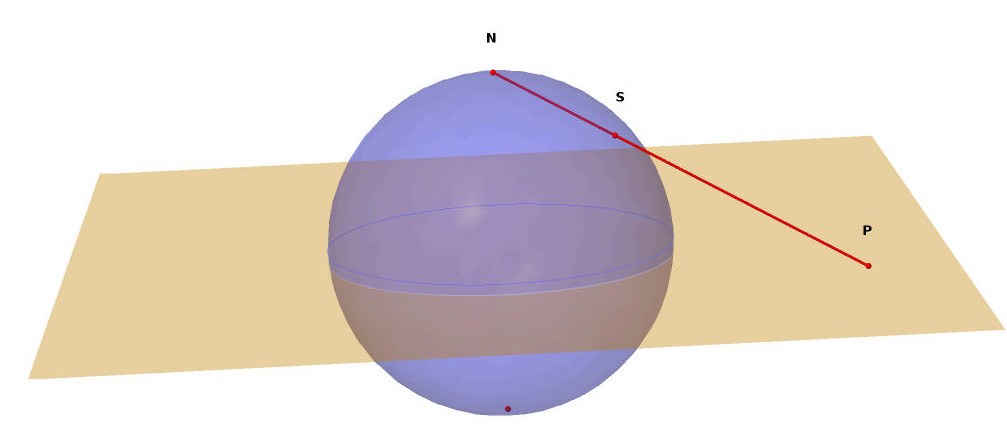
\includegraphics[scale=0.3]{figures/stereo1bis.jpg} 
\end{center}

  Le vecteur $\vect{NP}$ est colinéaire au vecteur $\vect{NS}$, il existe donc
  $k\in \Rr$ tel que  $\vect{NP} = k \vect{NS}$. Mais on veut de plus que
  $P$ appartienne au plan $\mathcal{P}$, c'est-à-dire $z_P = 0$. Ce qui permet de trouver $k$
  et d'en déduire $P = N + k\vect{NS}$. 
  On laisse \Sage\ faire les calculs :
 \insertcode{algos/stereographic-tex1.sage}{stereographic.sage (1)}
 
  On obtient $k = \frac{1}{1-z}$. Ainsi, si $S=(x,y,z)$ alors
  $P = \left( \frac{x}{1-z}, \frac{y}{1-z}, 0 \right)$.
  En identifiant les points du plan à $\Rr^2$, on a ainsi prouvé 
  $\Phi(x,y,z) = \left( \frac{x}{1-z}, \frac{y}{1-z} \right)$.
  D'où la définition de la fonction $\Phi$ : 
\insertcode{algos/stereographic-tex2.sage}{stereographic.sage (2)}  

  \item Voici la fonction $\Psi$ :
\insertcode{algos/stereographic-tex3.sage}{stereographic.sage (3)}  
  
  On profite du fait que l'on nous donne le candidat, 
  pour se contenter de vérifier que c'est bien la bijection réciproque, c'est-à-dire
  $\Phi\big( \Psi(X,Y) \big) = (X,Y)$ pour tout $(X,Y) \in \Rr^2$.
  La composition s'écrit
\insertcode{algos/stereographic-tex4.sage}{stereographic.sage (4)}
 et comme alors \codeinline{newX} vaut \codeinline{X} et que \codeinline{newY} vaut \codeinline{Y}, cela prouve le résultat.
 
 Il est possible de composer les fonctions de plusieurs variables, mais il faut rajouter
 une \og\codeinline{*}\fg\ devant la fonction à composer :\\
 \centerline{\codeinline{stereo(*inverse_stereo(X,Y)))}}
 cela renvoie \codeinline{X,Y} ce qui prouve bien 
  $\Phi\big( \Psi(X,Y) \big) = (X,Y)$.
  L'opérateur \og\codeinline{*}\fg\ devant une liste permet de la décompacter, par exemple
  \codeinline{*(2,5,7)}  s'interprète comme \codeinline{2,5,7} qui peut alors être passé en argument à une fonction.
  
  Pour prouver $\Psi\big( \Phi(x,y,z) \big) = (x,y,z)$, il faudrait se souvenir
  que $(x,y,z) \in \mathcal{S}$ et donc que $x^2+y^2+z^2=1$.
 
  \item et 4. Voici comment tracer les courbes.
  La courbe du plan est tracée comme une ligne polygonale,
  avec un pas assez petit. Ensuite on calcule l'image par 
  $\Psi$ de chacun de ces points.
  
 \insertcode{algos/stereographic-tex5.sage}{stereographic.sage (5)} 
 
 Par exemple \codeinline{G = courbes(t^3,t^2,-2,2)} puis \codeinline{G.show()} trace la courbe
 du plan d'équation paramétrique $\big(t^3,t^2\big)$, $t\in[-2,2]$, ainsi
 que son image par la projection stéréographique inverse.
 
 Voici le cas d'un cercle et d'une droite du plan qui se coupent à angle droit. On visualise qu'il en est 
 de même pour les cercles de la sphère.
 

\begin{center}
  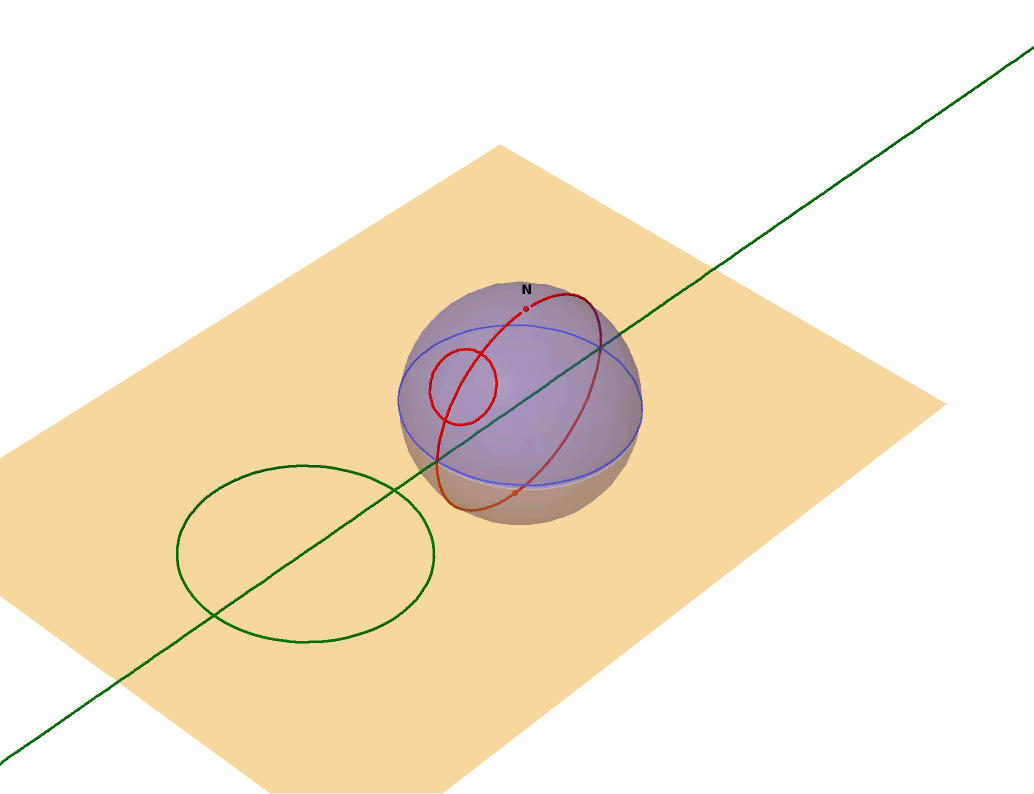
\includegraphics[scale=0.3]{figures/stereo2.jpg} 
\end{center}

\setcounter{enumi}{4}
  \item Voici une loxodromie de la sphère, courbe utilisée par les navigateurs, car elle
  correspond à une navigation à cap constant.
  

\begin{center}
  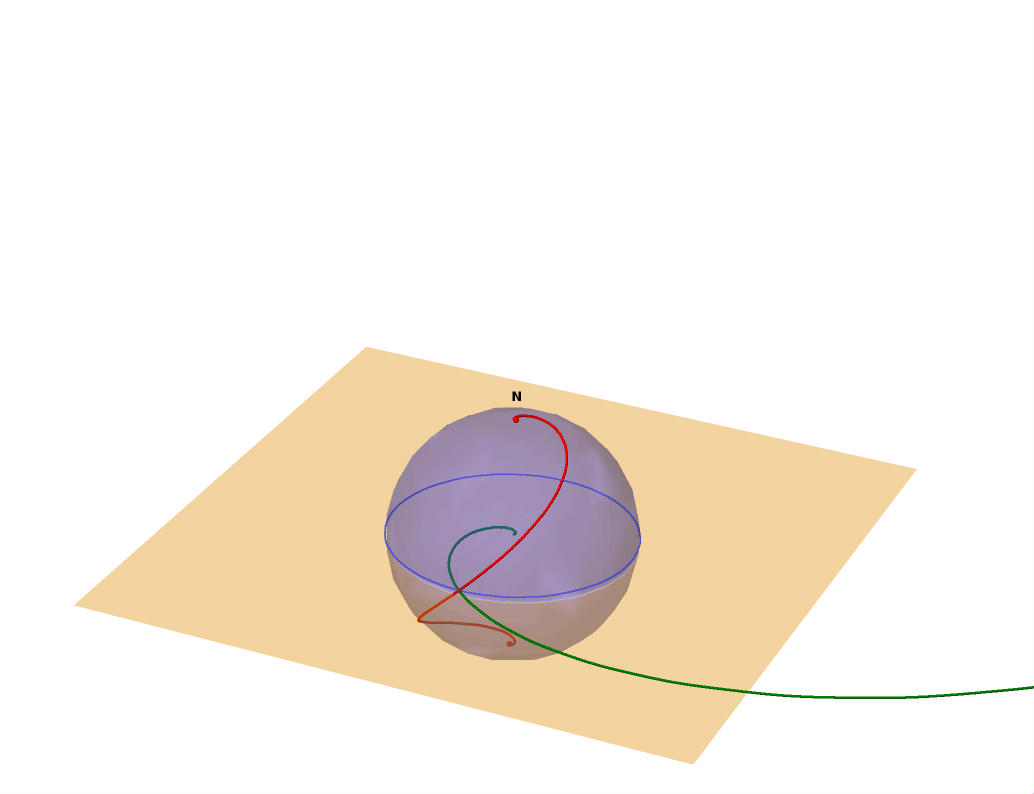
\includegraphics[scale=0.3]{figures/stereo3.jpg} 
\end{center}

  \item Pour $x,y,z$ définis par la paramétrisation, on calcule l'image par la projection stéréographique
  à l'aide de \codeinline{X,Y = stereo(x,y,z)}, on n'oublie pas de simplifier à l'aide de 
  \codeinline{full_simplify()}. Cela donne une paramétrisation de l'image,
  $x(t) = 2t$, $y(t) = -3t + 1$, qui est bien l'équation d'une droite.
  
\end{enumerate}

\finchapitre

\end{document}

